\documentclass[border=5mm]{standalone}
\usepackage{tikz}
\usetikzlibrary{positioning}
\usepackage{xcolor}
\usetikzlibrary{shapes,arrows}
\usetikzlibrary{trees}
\usetikzlibrary{shadows.blur}
\usetikzlibrary{decorations.pathmorphing}
\usetikzlibrary{decorations.markings}
\usetikzlibrary{intersections, calc}
\def\jt#1{\ensuremath{j_{\rm T#1}}}
\begin{document}
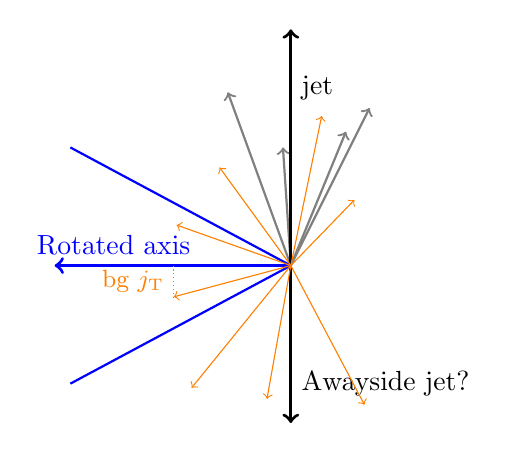
\begin{tikzpicture}
\draw[gray, thick, ->] (0,0) -- (1,2);
\draw[gray, thick, ->] (0,0) -- (-0.8,2.2);
\draw[gray, thick, ->] (0,0) -- (-0.1,1.5);
\draw[gray, thick, ->] (0,0) -- (0.7,1.7);
\draw[blue, thick] (0,0) -- (-2.8,1.5);
\draw[blue, thick] (0,0) --  (-2.8,-1.5);
\draw[blue, very thick, ->] (0,0) -- node [near end, above] {Rotated axis} (-3,0);
\draw[black, very thick, ->] (0,0) -- node [near end,right] {jet} (0,3);
\draw[black, very thick, ->] (0,0) -- node [near end, right] {Awayside jet?} (0,-2);
\draw[orange, thin, ->] (0,0) -- (-1.25982281336992,-1.55333398820495);
\draw[orange, thin, ->] (0,0) -- (-1.45147226001971,0.514614689251372);
\draw[orange, thin, ->] (0,0) -- (-0.30285006631157,-1.69312782663775);
\draw[orange, thin, ->] (0,0) -- (0.8074529522207,0.832838357636147);
\draw[orange, thin, ->] (0,0) -- (-1.48782136581293,-0.397476519344932);
\draw[orange, thin, ->] (0,0) -- (0.935437036685518,-1.76775494636474);
\draw[orange, thin, ->] (0,0) -- (-0.905166754522554,1.2459025429411);
\draw[orange, thin, ->] (0,0) -- (0.392170769946368,1.89994791697027);
\draw[orange, thin, densely dotted] (-1.48782136581293,0) -- node [midway, left] {\small bg $\jt{}$} (-1.48782136581293,-0.397476519344932);
\end{tikzpicture}
\end{document}